%%%%%%%%%%%%%%%%%%%%%%%%%%%%%%%%%%%%%%%%%%%%%%%%%%%%%%%%%%%
%%%                                                     %%%
%%%   LaTeX template voor P&O: Computerwetenschappen.   %%%
%%%                                                     %%%
%%%   Schrijfopdracht 2                                 %%%
%%%                                                     %%%
%%%   9 oktober 2013                                    %%%
%%%   Versie 1.1                                        %%%
%%%                                                     %%%
%%%%%%%%%%%%%%%%%%%%%%%%%%%%%%%%%%%%%%%%%%%%%%%%%%%%%%%%%%%

\documentclass{peno-opdracht2}
\usepackage{graphicx}
\setlength\parindent{0pt}
\team{Indigo} % teamkleur

\begin{document}

\maketitle

Nu de opdracht en planning van dit project duidelijk is, zullen we in detail treden over de hardware- en softwarecomponenten. 
\paragraph{Hardware} ~\\
Alle onderdelen van de zeppelin zullen gemonteerd worden op een frame. Hierop worden 3 propellers bevestigd. Hiervan worden er twee gebruikt om naar links en rechts te draaien. Om vooruit te bewegen worden deze samen geactiveerd met dezelfde kracht. De derde propeller dient om de zeppelin te laten stijgen. ~\\

Om het geheel in de lucht te houden, worden er 2 ballonnen gebruikt. Deze hebben een diameter van ongeveer 90 centimeter en bevatten helium. \\
\\
De zeppelin wordt aangestuurd door een Raspberry Pi model A. (zie Figuur \ref{Pi}) Deze heeft volgende specificaties: 
\begin{itemize}
	\item \emph{Processor:} 700MHz ARM
	\item \emph{Geheugen:} 256MB 
	\item \emph{Poorten:} 1 USB 2.0, HDMI, audio out, RCA video
	\item \emph{Voeding:} Micro USB
	\item GPIO-pinnen om de hardware aan te sturen
\end{itemize}

In de Raspberry Pi zit een SD-kaart van 4 GB. Op de USB-poort is een USB hub aangesloten, zodat het mogelijk is meerdere onderdelen aan te sluiten. Deze gebruiken we voor een toetsenbord, muis en WiFi dongle. \\

Verder zijn er nog 2 devices waarvan de zeppelin gebruik maakt:
\begin{itemize}
	\item De camera laat toe foto's te nemen met een maximum resolutie van 5 MP. Hiermee kunnen we onder andere beelden maken van QR-codes. Daarnaast kan de camera video's maken met resoluties tot 1080p. 
	\item De afstandssensor kan worden gebruikt om de afstand te meten tussen de zeppelin en de grond of muur. Het maximale bereik is 4m en het minimale bereik is 2cm.\\
\end{itemize}

\begin{figure}[ht!]
\centering
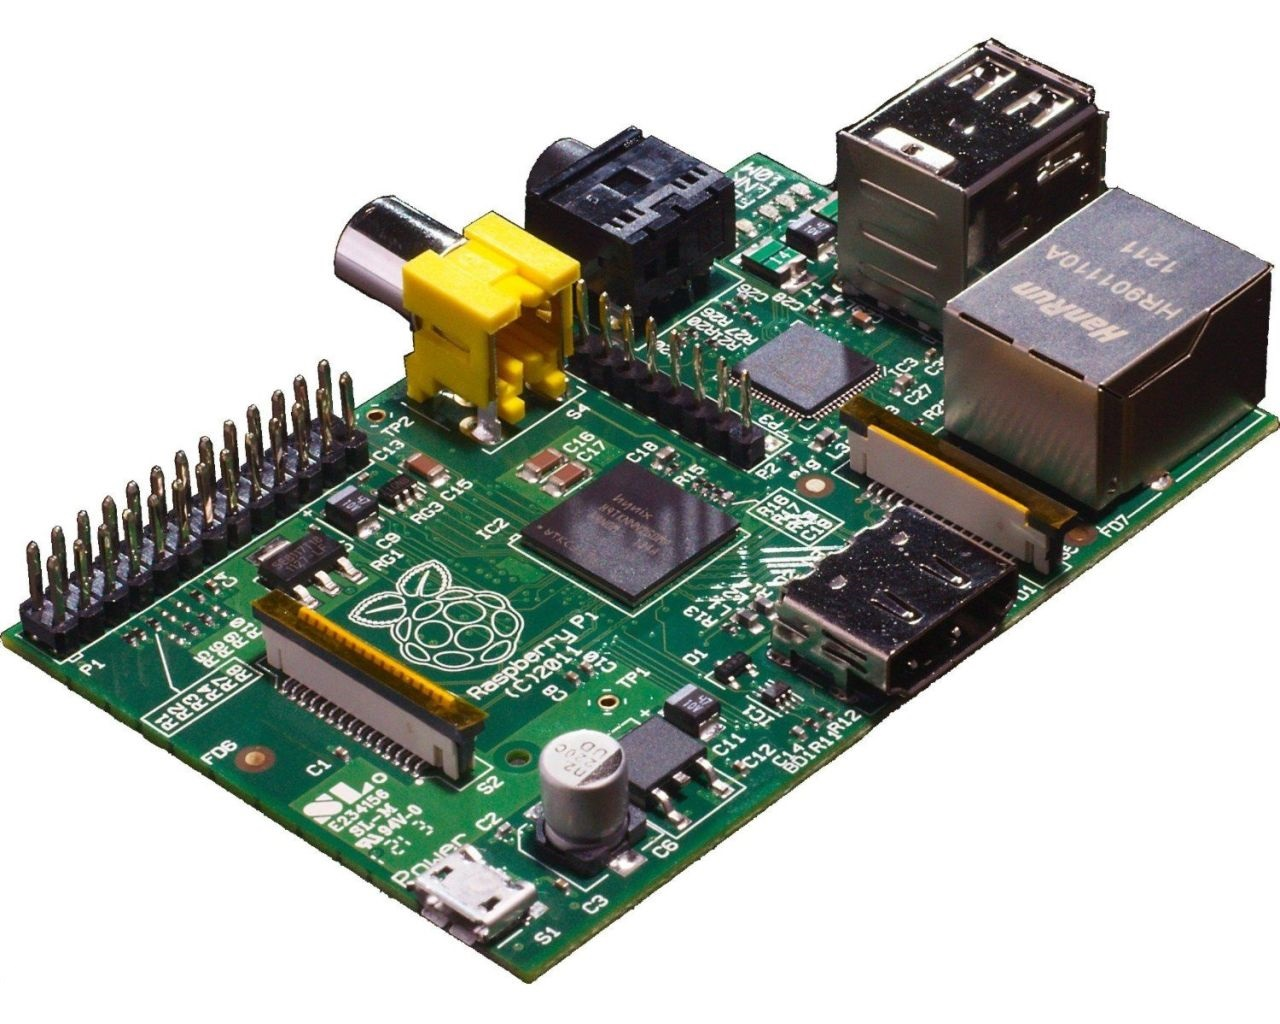
\includegraphics[height=30mm]{raspb.jpg}
\caption{Raspberry Pi}
\label{Pi}
\end{figure}

\paragraph{Software} ~\\
Zoals reeds vermeld, zal de software volledig in Java geschreven zijn. Deze keuze hebben we gemaakt omdat we al veel ervaring hebben met het schrijven van Java-programma's. Python was een andere mogelijke keuze. Er is veel voorbeeldcode in Python te vinden voor de Raspberry Pi, maar we hebben voor de functies die wij nodig hebben voldoende kennis en referenties in Java gevonden. Het leren van een extra taal zou erg tijdrovend in verhouding met de voordelen die het brengt. \\

Om de software te schrijven, gaan we op de laptop gebruik maken van de Eclipse IDE. We maken ook gebruik van de Netbeans IDE. Deze is door de visuele interface veel gebruikvriendelijker om de GUI te ontwerpen. Hierdoor moeten we ons niet bezig houden met alle code voor de lay-out handmatig te schrijven. Voor het aansturen van de GPIO-pinnen gebruiken we Pi4J\footnote{www.pi4j.com}.\\

Op een client-pc kan de GUI(zie figuur \ref{GUI}) worden gestart. Hiermee kan de gebruiker de zeppelin aansturen via de pijltjestoetsen. Deze commando's worden doorgestuurd aan de zeppelin om te verwerken. Op de GUI kan de gebruiker informatie aflezen zoals de hoogte en afbeeldingen van de camera. \\

De communicatie tussen de GUI (client) en de Raspberry Pi (server) gebeurt via sockets. Dit is zoals een deur waarlangs objecten van klassen uitgewisseld worden. Deze stellen bijvoorbeeld commando's van de gebruiker voor of de status van de zeppelin die aan de GUI wordt doorgegeven. Concreet opent de server een socket op poort 6789 (de eerste 1024 poorten zijn gereserveerd voor services zoals http en ftp, we hebben een willekeurige poort hierachter gekozen). Hierop kan 1 client verbinden. Het zou mogelijk zijn meerdere clients toegang te geven, maar om conflicten (met pijltjestoetsen) te vermijden en om bandbreedte te besparen (bij het doorsturen van afbeeldingen), ondersteunt de server maar 1 client.  \\

Om meerdere taken tegelijk te kunnen uitvoeren, maken we gebruik van threads. Zo kan de zeppelin tegelijk foto's nemen en de afstand tot de grond meten. Later zal worden beslist hoeveel gelijklopende threads er gebruikt worden. \\

Alle software behalve de GUI draait op de Raspberry Pi, omdat die autonoom moet kunnen werken. Hier worden beslissingen genomen op basis van QR-codes, die uit afbeeldingen komen die de camera op geregelde tijdstippen neemt. Elke opname van de camera wordt ook naar de GUI doorgestuurd. Het verwerken van de beelden zal gebeuren op de Raspberry Pi. Logisch gezien is het weergeven van de status van de zeppelin echter geen taak van de Pi zelf. Daarom draait de GUI op de client. Daarnaast wordt door deze keuze de CPU van de Pi minder zwaar belast. \\

De hoogte zal ook op bepaalde momenten opgemeten worden. Om een zo accuraat mogelijke waarde te krijgen, wordt de mediaan genomen van een aantal opeenvolgende meetresultaten. De hoogte wordt, net zoals de foto's, doorgestuurd naar de GUI.

\begin{figure}[ht!]
\centering
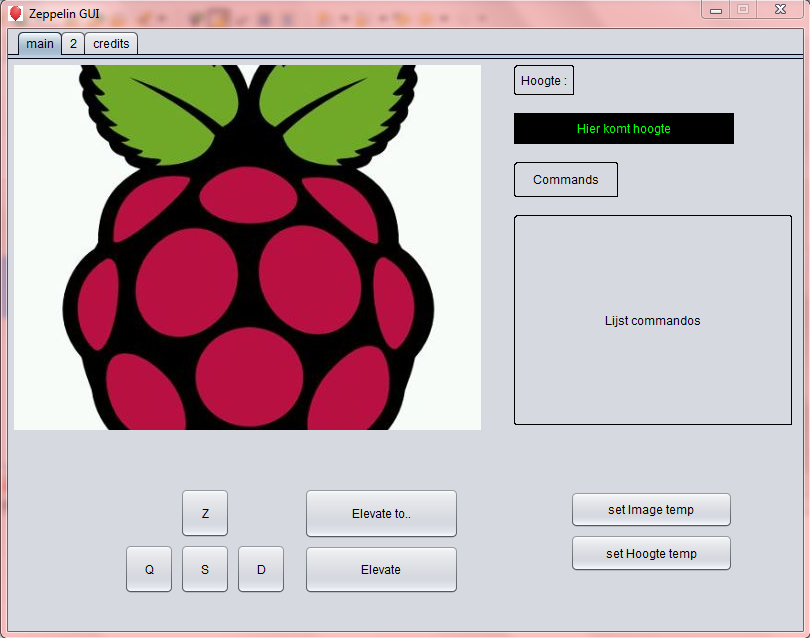
\includegraphics[height=40mm]{GUI.png}
\caption{GUI}
\label{GUI}
\end{figure}


\paragraph{Opmerking} ~\\
Omdat we nog niet beschikken over alle nodige hardware, is het op dit moment onmogelijk om dieper in te gaan op de softwarematige aansturing van de motoren. In een latere fase van het project zal dit verder uitgewerkt worden.

\end{document}
